%Introduction:

%Briefly explain what an accelerator is and its importance in scientific research
The Proton Synchrotron (PS) is part of the injector chain and is used to accelerate particles from the Proton Sychrotron Booster (PSB) to the SPS and finally to the Large Hadron Collider (LHC). For the purpose of CHIMERA, it can also be receive and accelerate heavy ions from the Low Energy Ion Ring (LEIR) and extract them to the East Area. The PS uses radio frequency (RF) cavities to accelerate charged particles, such as protons or Pb ions, to high energies and uses 100 dipoles to bend the beam around its 628 m circumference \cite{}. These particles are then extracted using slow extraction through a beam line and transported to the CHARM facility, where the CHIMERA instruments are located.

%Introduce the concept of beam energy and its significance in the operation of an accelerator
The beam energy refers to the kinetic energy per nucleon $E_{kin}$ of the charged particles beam. The relationship for an ion beam is $E_{kin, TOT}=E_{kin}\cdot A$, where A is the atomic mass number (A = Z + N, the number of protons Z and neutrons N). The total momentum for an ion beam is \cite{chao_handbook_2013}

$$pc={E_{0}\sqrt{\gamma^{2}-1}}$$

$$pc = E_{0}\sqrt{\left [ \left( \frac{E_{kin}}{E_{0}}+1\right )^{2}-1\right ]}$$

where, $E_{0}$ is the rest mass of the ion and $\gamma=\frac{E}{E_{0}}=\frac{E_{0}+E_{cin}}{E_{0}} = \frac{E_{cin}}{E_{0}}+1$

The rigidity is defined as and will be used to calculate the magnetic field used in the bending magnets of the PS:
$$B\rho = \frac{pc}{q}$$

The CHIMERA beam uses a lead ion beam. During its acceleration, it is a Pb54+ ion beam of partially stripped electrons (which means that it has 54 charges and 28 $e^{-}$ remaining) of isotope A=208. As an example for a 1 GeV per nucleon, the momentum would be:

$$pc = E_{0}\sqrt{\left [ \left( \frac{1\text{ [GeV]}\cdot 208}{E_{0}}+1\right )^{2}-1\right ]}$$

where the rest mass $E_{0}$ of Pb54+ is \cite{boston_university_nuclear_nodate}:

$$E_{0} = m_{Pb54+}= 82\cdot m_{proton} + 126\cdot m_{neutron} + 28\cdot m_{e^{-}} - m_{defect} = 193.74 \frac{\text{GeV}}{\text{c}^{2}}$$

with the mass defect: $m_{defect}=82\cdot m_{proton} + 126\cdot m_{neutron} + 28\cdot m_{e^{-}} - 208\cdot m_{u}$ 

%$$m_{p} = 0.93828 \text{ } GeV/c^{2}$$
%$$m_{n} = 0.93957 \text{ } GeV/c^{2}$$
%$$m_{e^{-}} = 0.000511 \text{ } GeV/c^{2}$$
%$$m_{u} = 0.9315 \text{ } GeV/c^{2}$$


The conversion of beam momentum to rigidity in Tesla meter is done with: 
$$B\rho \text{ [T m]} = 3.3356\cdot p \text{ [GeV/c]}$$
where for the PS, $\rho = 70.0789$ m.

For the ESA run we selected three energies and calculated the magnetic field (B-field) to which the ions will be accelerated to, see Fig. \ref{fig:lookup table}.

\begin{figure}[!htb]
\centering
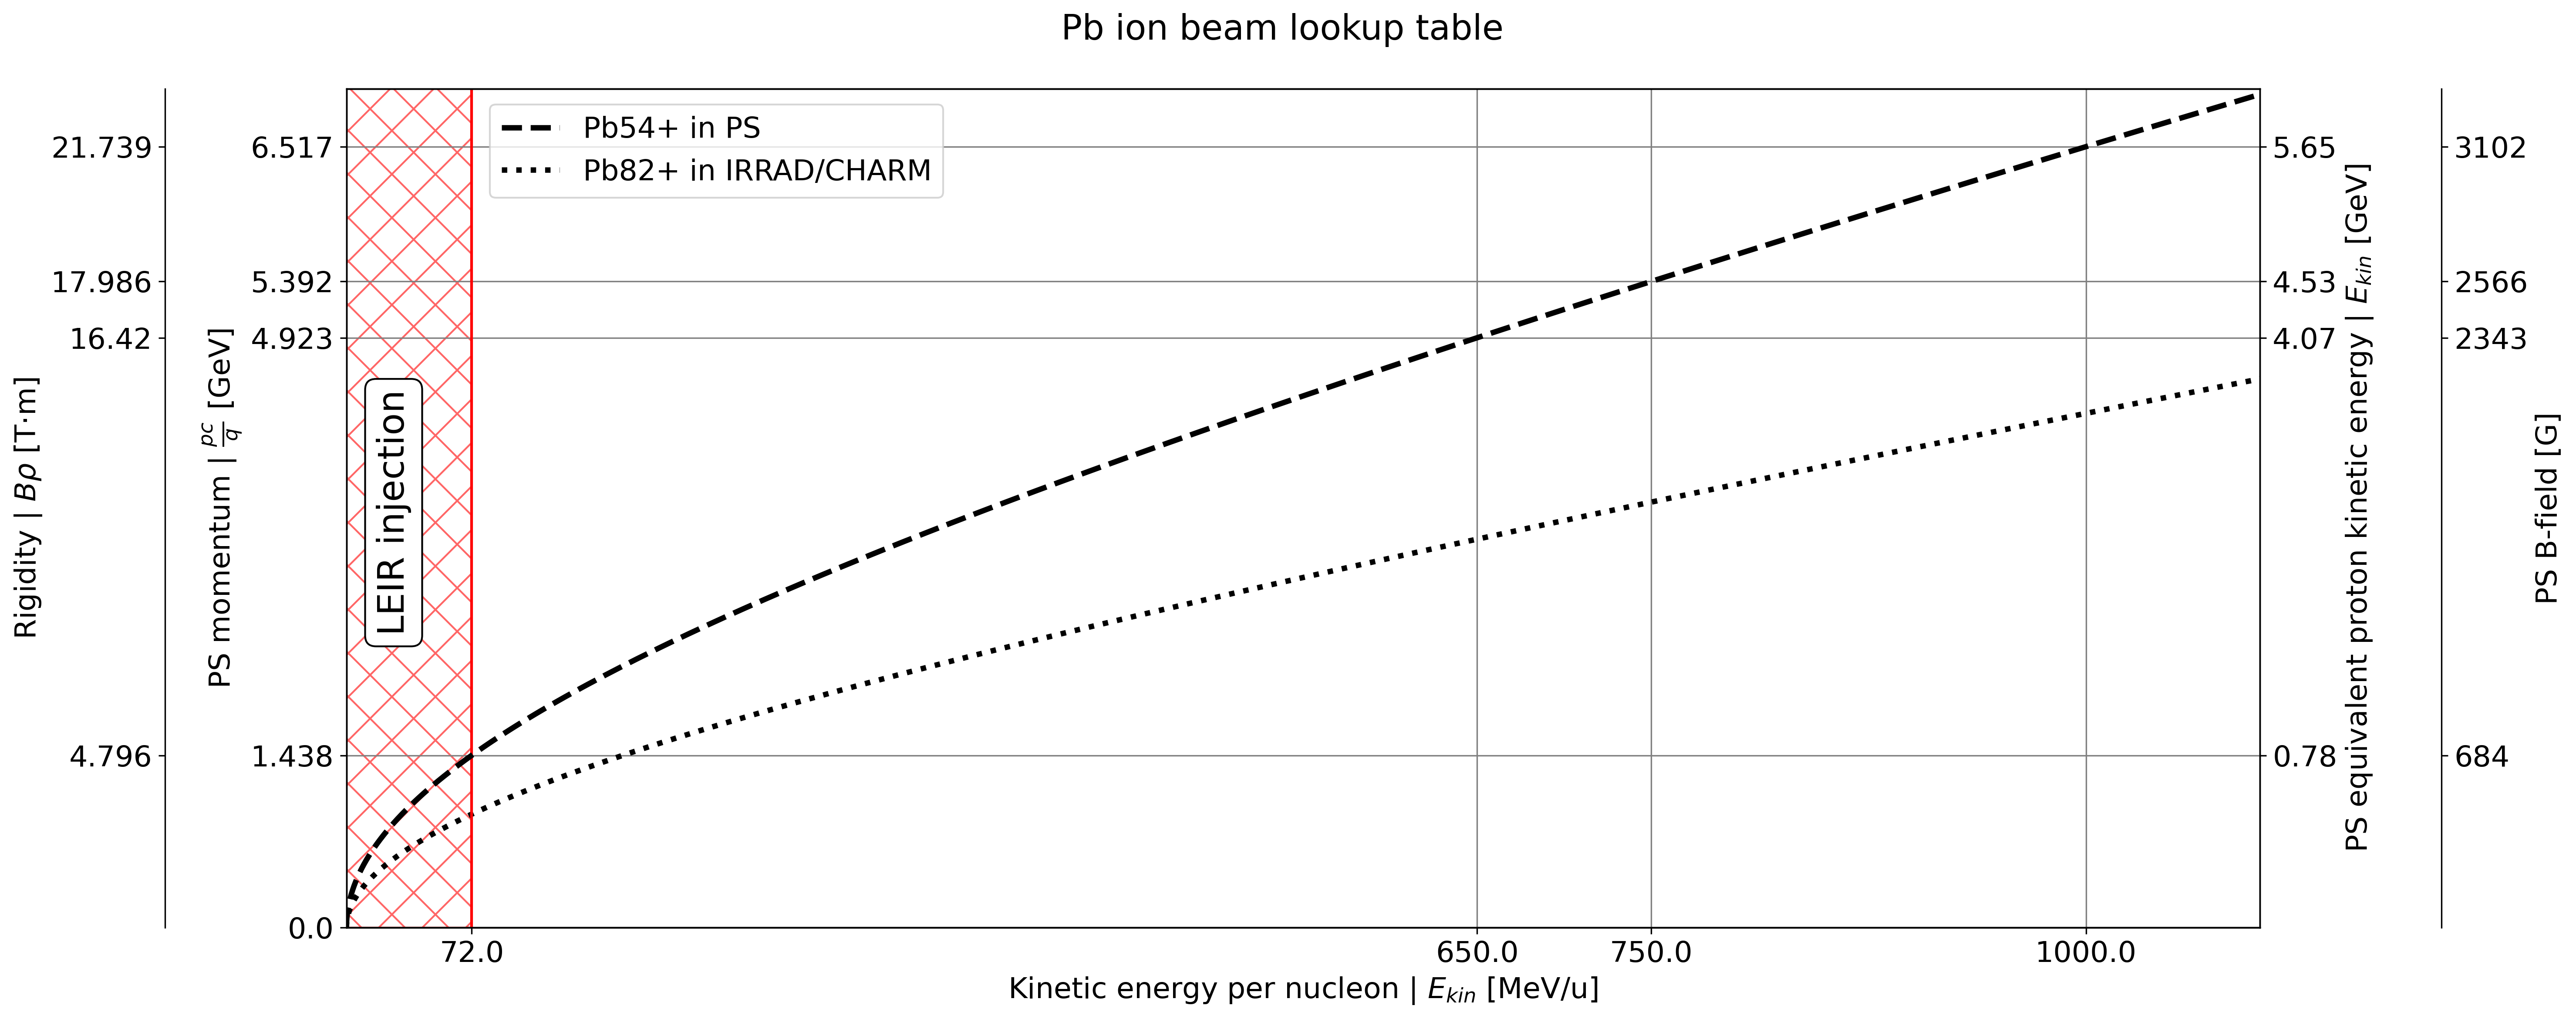
\includegraphics[width=1.0\textwidth]{images/kinetic_energy_lookup_table_zoom_B_field.png}
\caption{Lead ion beam lookup table}
\label{fig:lookup table}
\end{figure}

Figure \ref{fig:bfield} shows the shape of the magnetic field in the main dipoles of the PS produced by the Power system for the PS main magnet (POPS). There are two main regions, the injection plateau and the flat-top extraction plateau. The spike at the end to circumvent some limitation of POPS should be disregarded as the extraction is done prior to this event.

\begin{figure}[!htb]
\centering
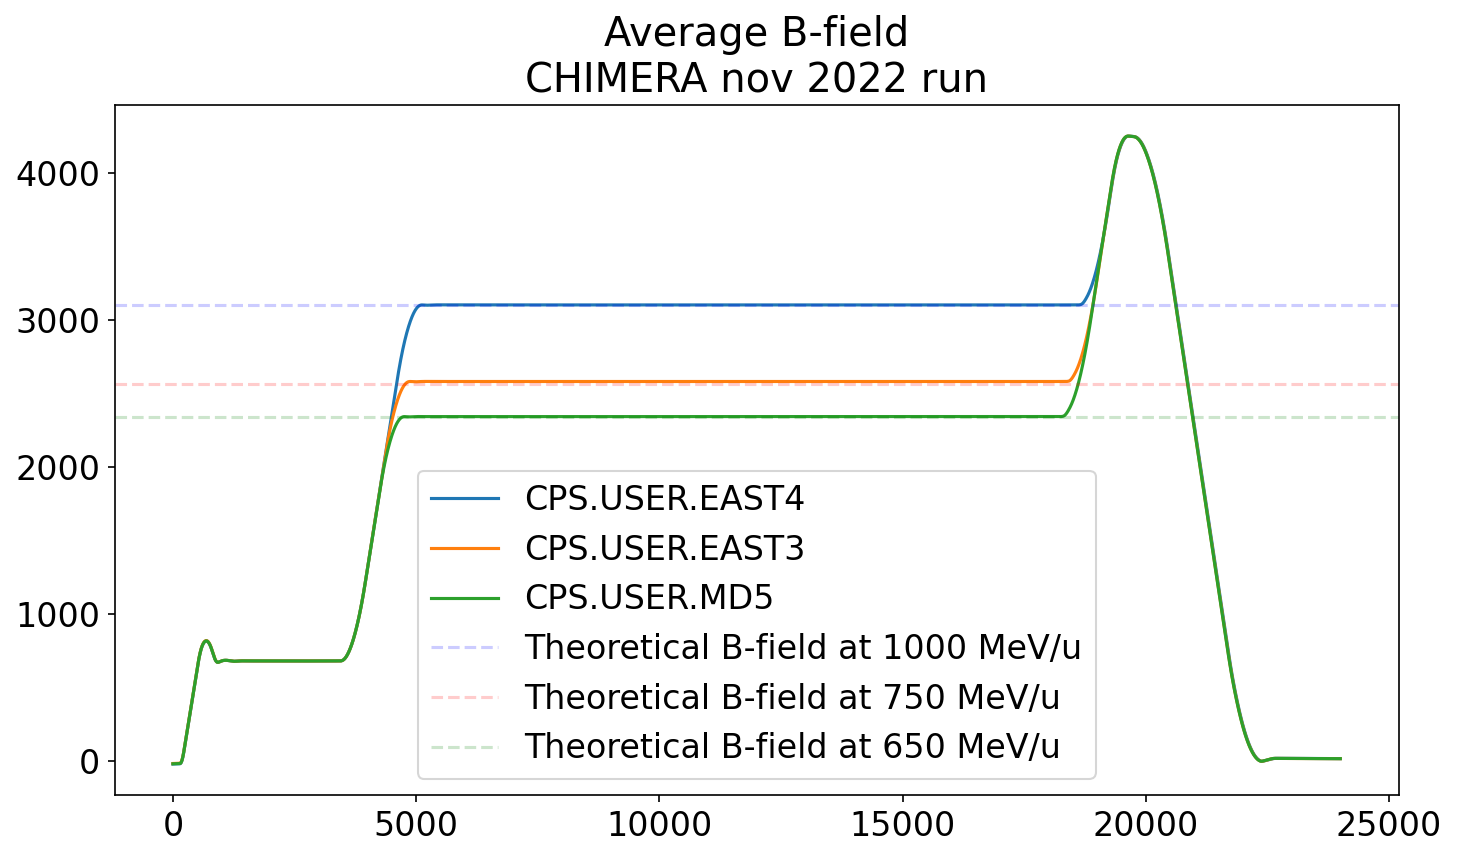
\includegraphics[width=0.6\textwidth]{images/average_b_field_chimera.png}
\caption{CHIMERA B-field for different energies. There are two plateaus: the injection plateau at 684 G and then extraction plateaus at different B-field corresponding to different energies.}
\label{fig:bfield}
\end{figure}

\begin{table}[h!]
\centering
\begin{tabular}{rrrr}
\toprule
 $E_{kin}$ [MeV/nucleon] &  $\frac{pc}{54}$ [GeV] &  $\frac{pc}{82}$ [GeV] &  PS B-field [G] \\
\midrule
  1000 &                        6.517 &                    4.292 &        3102 \\
   750 &                        5.392 &                    3.551 &        2566 \\
   650 &                        4.923 &                    3.242 &        2343 \\
    72 &                        1.438 &                    0.947 &         684 \\
\bottomrule
%\caption{Lead ion beam lookup table}
\label{fig:lookup table}
\end{tabular}
\caption{Kinetic energy table.}
\label{table:KE_table}
\end{table}

\begin{figure}[!htb]
\centering
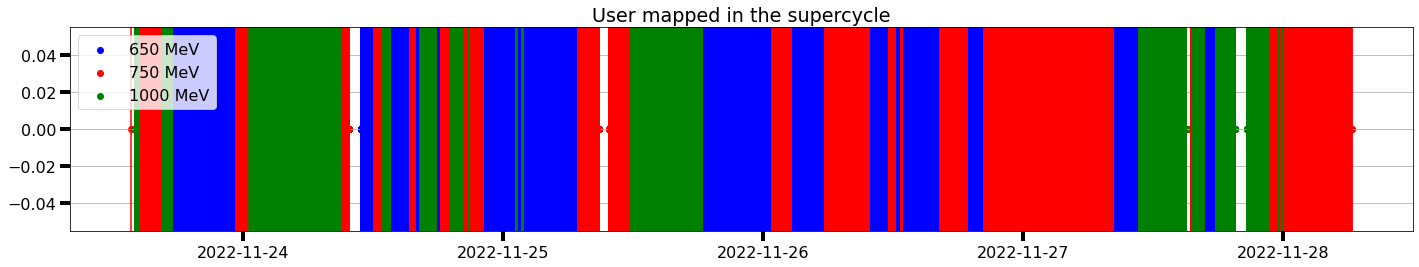
\includegraphics[width=1.0\textwidth]{images/Pasted image 20221130110611.png}
\caption{Timestamp of different energies}
\label{fig:timestamp_energies}
\end{figure}

\subsubsection{Energy scan}

For development purposes and after the ESA run, we ramped the beam energy using an automatic script.

\begin{figure}[!htb]
\centering
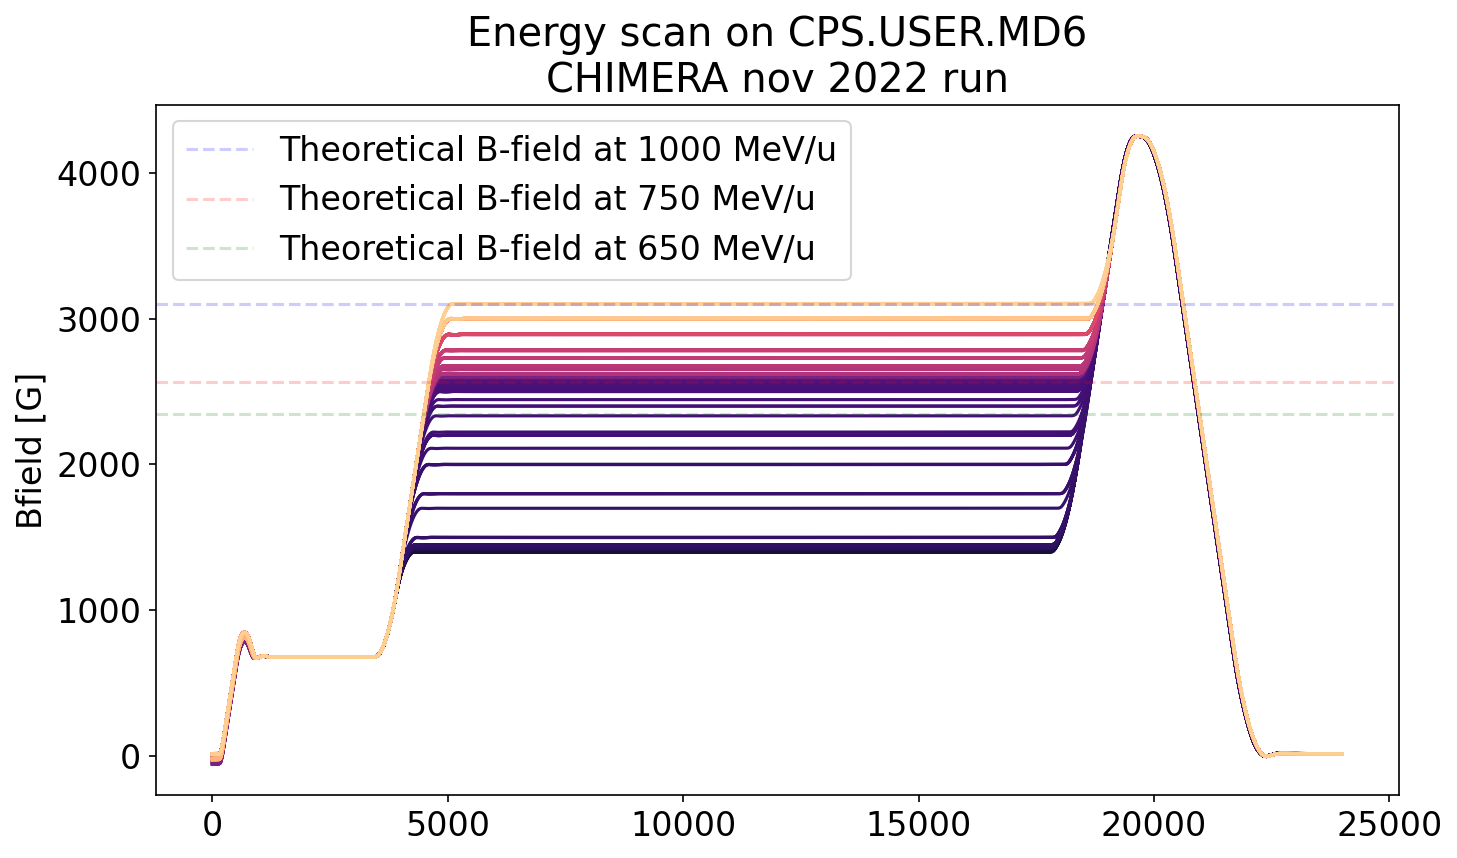
\includegraphics[width=0.6\textwidth]{images/energy_scan_chimera 1.png}
\caption{Energy scan}
\label{fig:energy_scan}
\end{figure}


\begin{figure}[!htb]
\centering
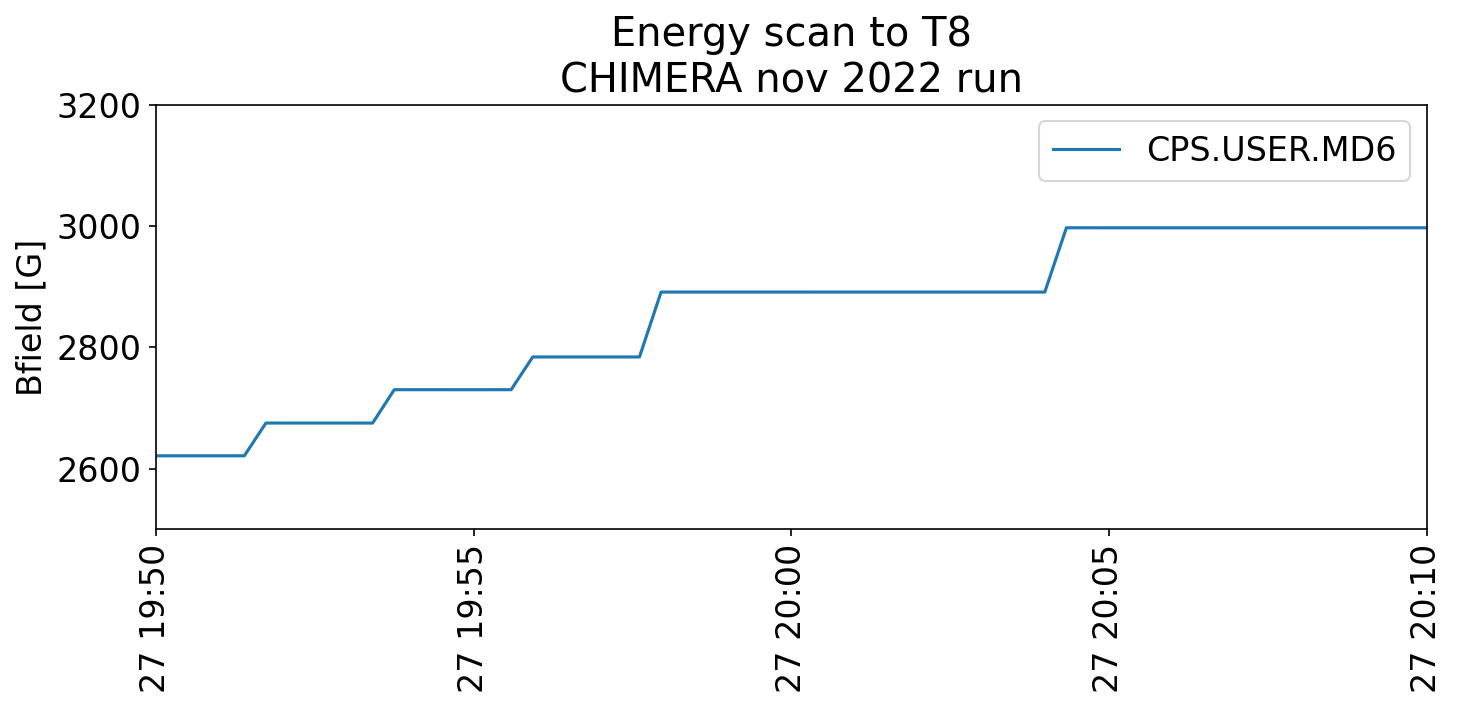
\includegraphics[width=0.6\textwidth]{images/energy_scan_timestamp_chimera 1.png}
\caption{Energy scan with timestamp}
\label{fig:energy_scan_timestamp}
\end{figure}
